%!TEX root = labreport.tex
%%%%%%%%%%%%%%%%%%%%%%%%%%%%%%%%%%%%%%%%%%%%%%%%%%%%%%%%%%%%%%%%%%%%%%%%%%%

\documentclass[sigconf]{acmart}

\usepackage{booktabs} % For formal tables
\usepackage{amsmath}

% Copyright
\setcopyright{none}
%\setcopyright{acmcopyright}
%\setcopyright{acmlicensed}
%\setcopyright{rightsretained}
%\setcopyright{usgov}
%\setcopyright{usgovmixed}
%\setcopyright{cagov}
%\setcopyright{cagovmixed}


% DOI
% \acmDOI{10.475/123_4}

% ISBN
% \acmISBN{123-4567-24-567/08/06}

%Conference
\acmConference[SEEMOO PhySec (Lab RDS) 2017/18]{Physical Layer Security
in Wireless Systems (Lab RDS) 2017/18}{February 2018}{Darmstadt, Germany}

\acmYear{2018}
\copyrightyear{2018}

% \acmArticle{4}
% \acmPrice{15.00}

\settopmatter{printacmref=false}

\begin{document}
\title{Radio Data Signal Transmission With Software Defined Radios}

% Comment out the following for you final document
\subtitle{Lab Report}



\author{Daniel May}
\author{Simon Schmitt}
\affiliation{%
  \institution{Technische Universtit\"at Darmstadt}
}
\email{daniel\_nicolas.may@stud.tu-darmstadt.de}
\email{simon\_johannes.schmitt@stud.tu-darmstadt.de}

% The default list of authors is too long for headers.
\renewcommand{\shortauthors}{Daniel May \& Simon Schmitt}


\begin{abstract}
%  Answer the following questions with roughly one sentence each:
%
%  One-page summary:
%  \begin{itemize}
%  \item What is the topic of your main seminar paper?
%  \item What problem does it solve?
%  \item Why is that topic/problem important?
%  \item What methodologies do the authors apply?
%  \item What are the main contributions of the paper?
%  \item What are the key findings/results of the paper?
%  \end{itemize}
%  
%  Final seminar paper:
%  \begin{itemize}
%  \item What is your research question?
%  \item Why are that question and your topic important?
%  \item How did you proceed to answer the question?
%  \item What (do you think) is the answer to your question?
%  \item Give an overall opinion on your topic.
%  \item If you have results, describe them.
%  \item What is the impact of the answers to your questions?
%  \end{itemize}
This lab report presents the creation and transmission of a Radio Data System signal.
The signal is generated on the basis of given sample data according to the corresponding
standard document. In the end, we could successfully receive and decode the signal
using a customary FM radio.


\end{abstract}

%
% The code below should be generated by the tool at
% http://dl.acm.org/ccs.cfm
% Please copy and paste the code instead of the example below. 
%
% \begin{CCSXML}
% <ccs2012>
%  <concept>
%   <concept_id>10010520.10010553.10010562</concept_id>
%   <concept_desc>Computer systems organization~Embedded systems</concept_desc>
%   <concept_significance>500</concept_significance>
%  </concept>
%  <concept>
%   <concept_id>10010520.10010575.10010755</concept_id>
%   <concept_desc>Computer systems organization~Redundancy</concept_desc>
%   <concept_significance>300</concept_significance>
%  </concept>
%  <concept>
%   <concept_id>10010520.10010553.10010554</concept_id>
%   <concept_desc>Computer systems organization~Robotics</concept_desc>
%   <concept_significance>100</concept_significance>
%  </concept>
%  <concept>
%   <concept_id>10003033.10003083.10003095</concept_id>
%   <concept_desc>Networks~Network reliability</concept_desc>
%   <concept_significance>100</concept_significance>
%  </concept>
% </ccs2012>  
% \end{CCSXML}

% \ccsdesc[500]{Computer systems organization~Embedded systems}
% \ccsdesc[300]{Computer systems organization~Redundancy}
% \ccsdesc{Computer systems organization~Robotics}
% \ccsdesc[100]{Networks~Network reliability}


% \keywords{ACM proceedings, \LaTeX, text tagging}


\maketitle

\section{Introduction}

Radio signals have been used for more than a century now, to broadcast
information wirelessly. The best known one is the FM radio, as it can be
received by everyone with a common radio receiver. While the FM radio was
originally developed to broadcast music and news reports from different
radio stations, more enhanced receivers allowed to process additional
information (e.g traffic updates in car radios) next to the existing
ones. Therefore, the \emph{Radio Data System (RDS)} was invented. 
In this lab report we will give a detailed insight into RDS and how it can be
implemented. We have divided the report into a preparation section, to discuss the
data that will be transmitted via RDS and several sections for the individual tasks we have solved. 

%Write a short paragraph (5-15 lines) on each of the following tasks:
%\begin{itemize}
%\item Motivate your topic in general.
%\item Why is your research question important in that field?
%\item Give one practical example.
%\item To what existing work is your topic related, what has been done there?
%\item What are the (planned) main contributions of your paper? e.g., a
%new attacker model, a summary, a comparison, \dots
%\item Give an outline of the paper: describe each of your (planned)
%sections in one sentence.
%\end{itemize}


%\section{Background and Related Work}

\section{Implementation}

In the following we describe how RDS signals can be generated using MATLAB.

\hypertarget{Preparation:ux20Basebandux20Coding}{%
\subsection{Preparation: Baseband
Coding}\label{Preparation:ux20Basebandux20Coding}}

Before the actual implementation we have to define and format the
information we are about to generate.

\begin{itemize}
%\tightlist % <-- hab ich mal auskommentiert weil das bei mir zu Problemen fuehrt
\item The programme service name should be ``\#SEEMOO\#''
\item We want to transmit a Mono signal without Artificial Head
\item The signal is not compressed
\item We use a static PTY which is set to Pop Music
\item We want to transmit Music
\item We do not carry traffic announcements
\item Our radio station is in Germany
\item We cover a local area
\item We use 1 as the program reference number
\end{itemize}

To be able to transfer this information it has to be converted into a binary stream using baseband
coding. The standard documentation\cite{rds_standard} of RDS defines that the stream of bits is split into
multiple groups. Each of them consists of four blocks, which have predefined meanings. Since, each
group can only transmit two symbols we need four groups to send the programme service name. The
overall encoding is shown in table\ref{tab:baseband_coding}.


\begin{table}[H]
\centering
\begin{tabular}{ l | c | c | c | r}
\hline
Group 1 Block 1 & 1 1 0 1 & 0 0 0 0 & 0 0 0 0 & 0 0 0 1\tabularnewline
Group 1 Block 2 & 0 0 0 0 & 1 0 0 1 & 0 1 0 0 & 1 0 0 0\tabularnewline
Group 1 Block 1 & 1 1 0 1 & 0 0 0 0 & 0 0 0 0 & 0 0 0 1\tabularnewline
Group 1 Block 4 & 0 0 1 0 & 0 0 1 1 & 0 1 0 1 & 0 0 1 1\tabularnewline
Group 2 Block 1 & 1 1 0 1 & 0 0 0 0 & 0 0 0 0 & 0 0 0 1\tabularnewline
Group 2 Block 2 & 0 0 0 0 & 1 0 0 1 & 0 1 0 0 & 1 0 0 1\tabularnewline
Group 2 Block 3 & 1 1 0 1 & 0 0 0 0 & 0 0 0 0 & 0 0 0 1\tabularnewline
Group 2 Block 4 & 0 1 0 0 & 0 1 0 1 & 0 1 0 0 & 0 1 0 1\tabularnewline
Group 3 Block 1 & 1 1 0 1 & 0 0 0 0 & 0 0 0 0 & 0 0 0 1\tabularnewline
Group 3 Block 2 & 0 0 0 0 & 1 0 0 1 & 0 1 0 0 & 1 0 1 0\tabularnewline
Group 3 Block 3 & 1 1 0 1 & 0 0 0 0 & 0 0 0 0 & 0 0 0 1\tabularnewline
Group 3 Block 4 & 0 1 0 0 & 1 1 0 1 & 0 1 0 0 & 1 1 1 1\tabularnewline
Group 4 Block 1 & 1 1 0 1 & 0 0 0 0 & 0 0 0 0 & 0 0 0 1\tabularnewline
Group 4 Block 2 & 0 0 0 0 & 1 0 0 1 & 0 1 0 0 & 1 0 1 1\tabularnewline
Group 4 Block 3 & 1 1 0 1 & 0 0 0 0 & 0 0 0 0 & 0 0 0 1\tabularnewline
Group 4 Block 4 & 0 1 0 0 & 1 1 1 1 & 0 0 1 0 & 0 0 1 1\tabularnewline
\hline
\end{tabular}
\caption{The Baseband Coding of \textit{\#SEEMOO\#}}
\label{tab:baseband_coding}
\end{table}

\hypertarget{Task1:ux20Bitstreamux20Generation}{%
\subsection{Task1: Bitstream
Generation}\label{Task1:ux20Bitstreamux20Generation}}

Within this first task we initialize the message we want to send.
Therefore, we import the bit stream we previously prepared and append
the corresponding checksum and offset. After decoding the message in the
first test we get the following output, which shows the hexadecimal,
binary and decoded representation.

\hypertarget{Decoderux20Output}{%
\paragraph{Decoder Output}\label{Decoderux20Output}}

\begin{verbatim}
d001_0de 094b_3e2 d001_372 4f23_212
1101_0000_0000_0001__00_1101_1110
0000_1001_0100_1011__11_1110_0010
1101_0000_0000_0001__11_0111_0010
0100_1111_0010_0011__10_0001_0010
00B (BASIC) - PI:D001 - PTY:
Pop Music (country:DE/LY/YU/__/__, area:Local, program:1)
==>#SEEMOO#<== -  -  -Music-STEREO - AF:p
\end{verbatim}

\hypertarget{Task2:ux20Differentialux20Encoding}{%
\subsection{Task2: Differential
Encoding}\label{Task2:ux20Differentialux20Encoding}}

Since we are about to use frequency modulation (FM) in one of the next
steps it is recommended to perform a differential encoding. The problem
with modulation is that a receiver of a signal can not determine the
logic assigned to a phase shift, as it might be introduced by the
wireless channel. Differential encoding provides unambiguous signal
reception, because the encoding of the data depends not only on the
current signal state (bit), but also on the previous one.
(\(y_i = y_{i-1} \bigoplus x\)).


\hypertarget{Task3:ux20Manchesterux20Encoding}{%
\subsection{Task3: Manchester
Encoding}\label{Task3:ux20Manchesterux20Encoding}}

\begin{figure}[tb!]
	\hfill
	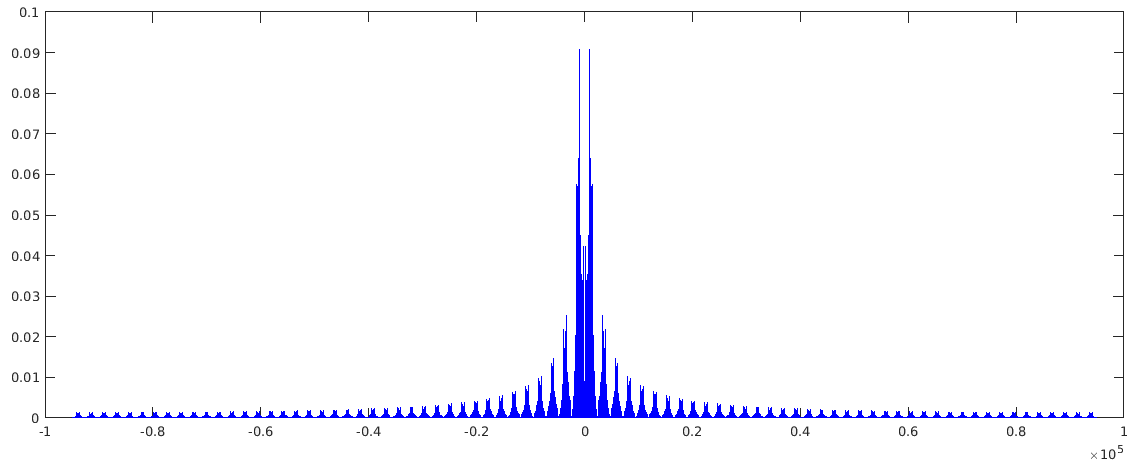
\includegraphics[width=1\linewidth]{rds_plot.png}
	\caption{RDS signal without lowpass filter.}
	\label{fig:rds_plot}
\end{figure}

\begin{figure}[tb!]
	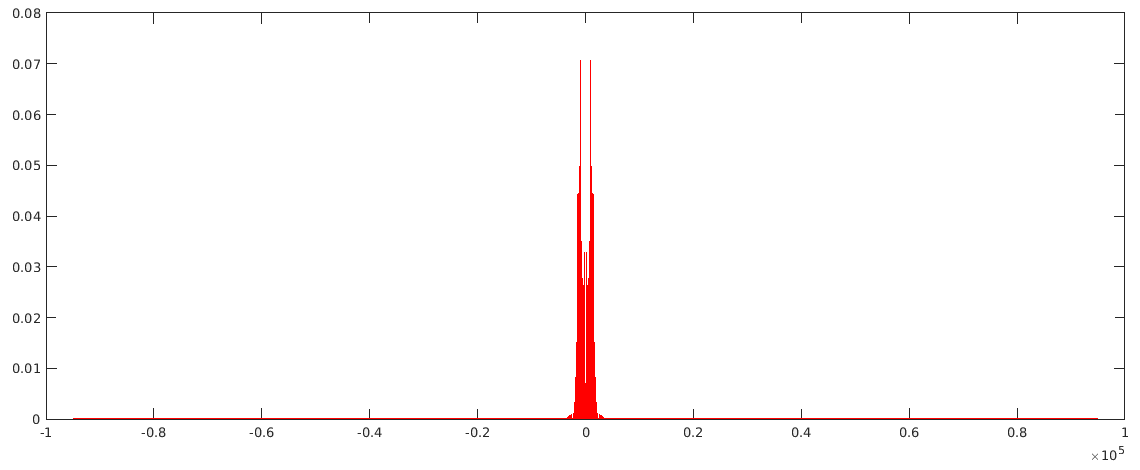
\includegraphics[width=1\linewidth]{rds_filt_plot.png}
	\caption{Lowpass filtered RDS signal.}
	\label{fig:rds_filt_plot}
\end{figure}

\emph{Manchester Encoding}, also called
\protect\hypertarget{Phaseux20Encodingux20ux28PEux29}{}{}\textit{Phase
Encoding (PE)}, is a line code. The information is represented by the
edge of a signal that corresponds to the clock. While we generate the clock signal in line 2 and 3
of the source code of Task3, Manchester Encoding is performed using the \textit{kron} functions starting at
line 6. A binary zero becomes a low to high transition, a
binary one a high to low transition. This type of representation is
named after G.E. Thomas \cite{tanenbaum1996computer}. After the differential encoded bitstream has
been mapped to Manchester Encoded symbols, we get a RDS signal. However,
as shown in Figure1 this signal also contains frequencies we actually
dont need. Therefore, we apply a lowpass filter and normalize the
resulting signal. This normalized signal is shown in Figure2.

\begin{verbatim}
 1 fprintf('Task 3: Manchester Encoding %.2f\n', toc);
 2 bit_clk = [ones(80,1);-ones(80,1)];
 3 bit_clk = repmat(bit_clk,
 4	     length(bitstream_differentially_encoded),1);
 5 
 6 rds = kron(bitstream_differentially_encoded, 
 7 	      [ones(80,1);-ones(80,1)]) ...
 8     + kron(~bitstream_differentially_encoded, 
 9	      [-ones(80,1);ones(80,1)]);
10 
11 f6 = fir1(300,2400/fs*2);
12 rds_filt = filter(f6,1,rds);
13 rds_filt = rds_filt/max(rds_filt);
\end{verbatim}

\hypertarget{Task4:ux20Generateux20Basebandux20Signal}{%
\subsection{Task4: Generate Baseband
Signal}\label{Task4:ux20Generateux20Basebandux20Signal}}

We will now generate the baseband signal. This signal represents the
actual data we want to transmit. First of all, we have to change the
frequency of the current signal to 57 kHz, since this is the expected
frequency for a RDS signal. Therefore, we multiply the RDS signal with a
57 kHz sine wave. To generate a complete baseband signal we also have to
insert a pilot and an audio signal. The pilot signal is generated with a
19 kHz sine wave and it is used to upconvert the RDS signal. The audio
signal is generated as a mono signal, which means that we sum up the
left and the right audio channel at a frequency of 0.3 to 15 kHz. The
spectrum of the final baseband signal is shown in Figure3.

\begin{figure}[tb!]
	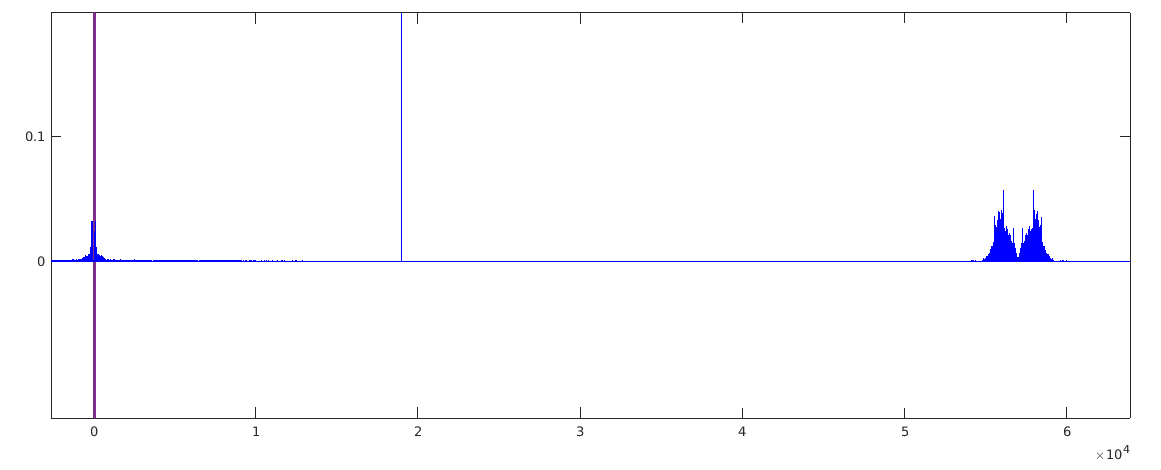
\includegraphics[width=1\linewidth]{baseband_spectrum2.png}
	\caption{Frequency spectrum of the baseband signal}
	\label{fig:rds_filt_plot}
\end{figure}

\hypertarget{Task5:ux20Frequencyux20Modulation}{%
\subsection{Task5: Frequency
Modulation}\label{Task5:ux20Frequencyux20Modulation}}
In software defined radios, the generated baseband signal we generated in Task4 is first frequency
modulated before it is upconvert to the carrier frequency. This is done by combining the carrier frequency
and the baseband signal and adapting the frequency according to the amplitude of the baseband signal.
In order to do the upconversion, a quadrature modulator is used. It seperately upconverts the inphase component
\[
I(t) = \cos (2 \pi f_\Delta \int_0^t m(\tau)\,\mathrm{d}\tau)
\]
by multiplication of a \( \cos(2 \pi f_c t) \) signal and the quadrature component
\[
Q(t) = \sin (2 \pi f_\Delta \int_0^t m(\tau)\,\mathrm{d}\tau)
\]
by multiplication of a \( -\sin(2 \pi f_c t) \)  signal. For readability reasons, we will
use the symbols \( \omega = 2 \pi f_c \) and \( \theta_m (t) = \int_0^t m(\tau)\,\mathrm{d}\tau \)
in the following. First, we calculate the upconversion of the inphase component
\begin{align*}
&\cos (2 \pi f_\Delta \theta_m (t)) \cdot \cos(\omega t)\\
&= \frac{1}{2}(\cos (2 \pi f_\Delta \theta_m (t) - \omega t) + \cos (2 \pi f_\Delta \theta_m (t) + \omega t))
\end{align*}
and second the upconversion of the quadrature component
\begin{align*}
&\sin (2 \pi f_\Delta \theta_m (t)) \cdot -\sin(\omega t)\\
&= \sin (2 \pi f_\Delta \theta_m (t)) \cdot \sin(-\omega t)\\
&= \frac{1}{2}(\cos (2 \pi f_\Delta \theta_m (t) + \omega t) - \cos (2 \pi f_\Delta \theta_m (t) - \omega t))
\end{align*}

These two signals are summed up to generate the complete signal that will still be amplified by the 
transmit amplifier and then sent. Thus we get 
\begin{align*}
&\frac{1}{2}(\cos (2 \pi f_\Delta \theta_m (t) - \omega t) + \cos (2 \pi f_\Delta \theta_m (t)+ \omega t))\\
&\hspace{1em}+ \frac{1}{2}(\cos (2 \pi f_\Delta \theta_m (t) + \omega t) - \cos (2 \pi f_\Delta \theta_m (t) - \omega t))\\
&= \frac{1}{2}(\cos (2 \pi f_\Delta \theta_m (t) - \omega t) + \cos (2 \pi f_\Delta \theta_m (t)+ \omega t)\\
&\hspace{1em}+ \cos (2 \pi f_\Delta \theta_m (t) + \omega t) - \cos (2 \pi f_\Delta \theta_m (t) - \omega t))\\
&= \frac{1}{2}(2 \cos (2 \pi f_\Delta \theta_m (t) - \omega t))\\
&= \cos (2 \pi f_\Delta \theta_m (t) - \omega t)
\end{align*}
Replacing the symbols from before again, we get the signal
\[
s'(t) = \cos (2 \pi f_c t + 2 \pi f_\Delta \int_0^t m(\tau)\,\mathrm{d}\tau)
\]
This can be combined into complex numbers by using the inphase component as real and the quadrature
component as imaginary part. Since we procress the signal digitally, we need it to be discrete which is
done achieved by sampling it and quantizing its amplitude. Applying this leads to the following frequency
modulated baseband signal, where the integral is replaced by a sum:
\[
fm_{BB} = exp(j2\pi f_\Delta T_s \sum_{k=0}^n m(kT_s))
\]

\begin{figure}[tb!]
	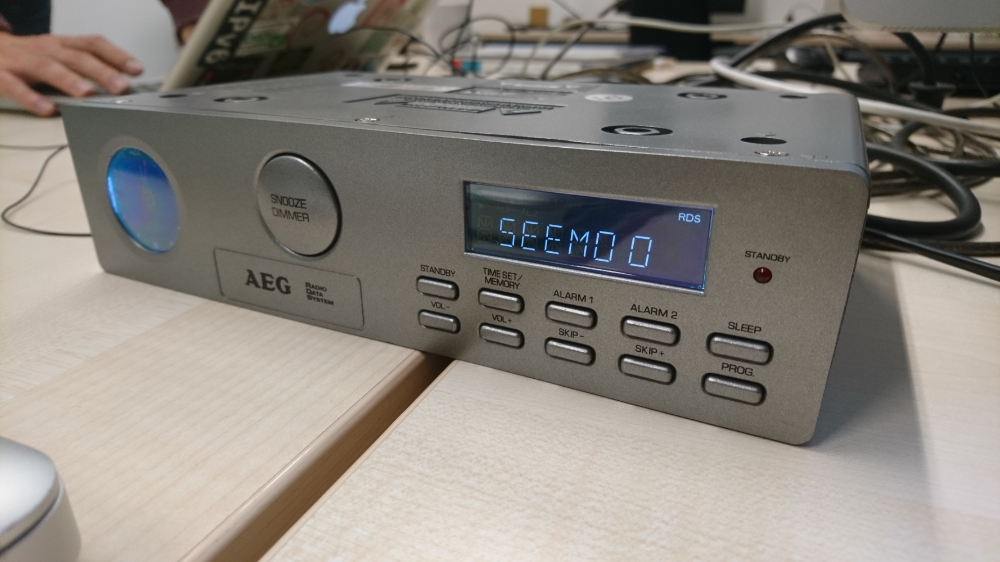
\includegraphics[width=1\linewidth]{radio_display.png}
	\caption{The FM radio after receiving our RDS signal.}
	\label{fig:rds_filt_plot}
\end{figure}


\hypertarget{Task6:ux20Transmission by USRPux20}{%
\subsection{Task6: Transmission by USRP}
\label{Task6:ux20Transmission by USRPux20}}
Finally, we setup a FM radio, connect to a USRP device and send the frequency modulated RDS signal.
As shown in Figure4 the FM radio receives and decodes the signal and displays the programme service
name \textit{\#SEEMOO\#} on the screen.

\section{Conclusion and Take-Away}
In this lab we generated and sent our own RDS Signal. We started from encoding the raw information
we wanted to transmit in text form to a binary form and further prepared this data for transmission by
applying a differential and a Manchester encoding. Then we generated the baseband signal, frequency
modulated and upconverted it and finally transmitted it using an USRP. The customary FM radio we used
to receive the signal showed the correct programme service name.\\
In the preparation for and during our work on this lab we learned how to build a RDS signal from the scratch
using the standard documentation. Furthermore we learned which mechanisms are used to ensure that
the receiver can decode the signal with as little loss of information as possible and how to implement them
using MATLAB. More precisely, we learned about the usage of the encoding schemes, the combination of
different signals and frequency modulation.

\section{Future Work}
Using this prototype implementation we could think of several questions one could investigate. First, is it
possible to send our own RDS signals to a driving car. Second, can existing RDS signals be manipulated
in any way, e.g. by jamming. Third, is there any possibility to overwrite the existing RDS signals sent by
real radio stations to accept our own data instead of the official one.
Moreover, the implementation could be extended by an additional module that also allows to receive
RDS signals using MATLAB. This module could be used to analyze RDS traffic in different locations.



\bibliographystyle{ACM-Reference-Format}
\bibliography{library} 

\end{document}
